\chapter{结合RFM与核密度估计的气井分类算法}
在气井开采初期,气井一经投入使用就会打破气藏的静态平衡,诸如产量、压力和产物性质等关键参数便会随之变动。随着开采活动的进行,气水关系会愈加错综复杂。产水量将持续攀升,
低压井和产水井的数量不断增长,不同气井之间的差异会日益增大。这些因素会进一步增加气井的生产管理难度。为提高管理效能,企业需利用历史产量数据对气井进行有效分类。将
表现出相似生产特性的气井进行归类和分析,以帮助揭示它们的共同生产模式。使得企业能够迅速评估气井的生产状况,掌握关键生产特征,进而及时规划出针对性强的管理策略和治
理行动,以确保气井的顺畅运作。本章使用了结合RFM与核密度估计的气井分类算法,根据根据气井的数据特征,对气井进行分类。首先对企业提供的报表数据进行整理和清洗,去除掉
报表中的冗余数据并将需要的信息批量提取出来。在获取了相应的气井信息后,使用结合RFM与核密度估计的气井分类算法来对气井进行分类。
\section{问题分析}
企业气田的地质条件十分复杂,是典型的“低渗透、低压力、低丰度”气田。其单井产量小、压降速率快,随着气田不断进行规模开发,单井井数逐年增加,集气站也在不断的增大。
随着开采活动的不断进行,间歇井(气井按照固定的开关制度进行生产的气井)数量的也在逐步递增。气井在开采过程中,产量会随着井底污染、地层压力、地层渗透率、地层有效厚度
等的变化。不同气井之间的特征差异较大,需要通过合理的方式对气井进行分类。常规砂岩气藏分类根据气井有效厚度、地层系数、孔隙度、渗透率、含气饱
和度、试气无阻流量、目前无阻流量、平均日产气量、单井稳产期配产、稳产时间、预测最终累计采气量为参数进行分类,需要通过分析各参数之间相关性寻找最
佳分类参数。本项目中初步想法是根据企业所提供报表数据,使用普通聚类算法如KMeans或者时间序列聚类算法如K-Shpae等对气井进行无监督分类。然而使用
这类聚类算法后发现该方法不具有稳定性,每次分类结果都不尽相同,无法达到向企业交付的标准。同时,对数据分布进行可视化展示以后,发现数据不是成团分布
,数据之间差异不大,不能简单地使用普通聚类算法。而采用K-Shpae进行时间序列聚类之后,发现不同类别之间无法提取出比较相似的特征,同一类别较为凌乱,
不能作为企业对气井分类的标准。经过分析发现普通的时间序列聚类算法大多是对过去时间序列的形状进行聚类,通过对K-Shape实验的数据结果\cite{Kshapeexperiment}
分析可以发现,其对于具有相似形状或模式的时间序列会有更好的分类效果,例如心跳、交通等具有相似周期性、趋势或季节性模式的时间序列。本文气井的时间序列没有
明显规律,因此其聚类效果较差。经过与企业专家讨论共同摸索,启发式的采用基于RFM\cite{birant2011data}评价参数和数据密度的分类方法来对气井进行分类。RFM模型是一种用于分析
客户价值和客户创收能力的方法,常用于数据库营销和直接营销中。将RFM模型应用于气井分类,可以充分挖掘气井的潜在价值。通过RFM模型来选取相应的参数,再根据数据的密度特征
选取相应的阈值,通过特征二值化的方法来对气井进行分类。

气井开采过程中,通常会产生一定量的液体,包括水和油。产液量的增加会影响气井的产气量,因为液体在井筒中的积累会增加井筒的阻力,使气流的速度降低,从而影响气井的产气量。当气井处于低压低产阶段时,气相不能有效地携带液体,会导致积液现象。此时,如采用间歇生产方式(即周期性地开关井),可以利用关闭期间积累的压力差,在开启时将积聚在底部或中部的液体迅速排出。
但如果开关频率过高或关闭时间过短,则可能造成反复积排液、增加摩阻损失、降低生产效率。可若是开关频率过低或关闭时间过长,则可能导致底部水锥突破、增加水含率、降低天然气质量。
\begin{figure}[H]
    \centering
    \caption{气井示意图}
\end{figure}
\section{问题描述}
在气井分类的问题中,本文的目标是将具有相似特征特征的气井分为一组,以帮助企业根据气井的特征更好地进行管理。此研究问题是提供某一气井相关数据,
确定其所属类别。问题的输入是气井的相关信息,单个数据可以表示为$x_i = \{x_{i1}, x_{i2}, \ldots, x_{iN}\}$,N表示特征数,输入数据集
$\mathbf{X} = \{X_{1}, X_{2}, \ldots, X_{m}\}$,m表示数据量的大小,输出是气井类别,将气井输出集表示为$\mathbf{Y}$,问题可以形式化为
求$\mathbf{X}$到$\mathbf{Y}$的一个映射$f$:$X \rightarrow Y$。
\section{算法框架}
\subsection{算法流程}\
\label{sec:K-Shapeprocess}
根据前文所述,传统的聚类方法以及基于时间的聚类方法在气井分类问题中效果较差,需要探寻一种合适的分类方法来对气井进行科学的分类。这其中的难点主要是
如何选取合适的分类模型以及合适的特征来对气井进行分类。本文采用在营销分析时常用的数据挖掘工具RFM模型来评估气井的价值。具体流程如图\ref{fig:wellcla}所示。
\begin{figure}
    \centering
    % Requires \usepackage{graphicx}
    \includegraphics[scale=0.15,angle=0]{}\\
    \caption{结合RFM与核密度估计的气井分类算法}
    \label{fig:K-Shape}
\end{figure}
在进行气井数据分析的初始阶段,面临着从原始报表中提取准确信息的挑战,该报表数据错综复杂且杂乱无章。为了转化这些数据为一份规范化的报表,首要步骤包括对原始数据进行细致的清理和整理工作。这一过程不仅涉及去除无关或重复的数据,还包括标准化数据格式和校正数据不一致性,以确保最终报表的数据质量和可靠性。

在构建规范化的数据框架之后,本文进一步利用RFM(Recency, Frequency, Monetary)模型作为分析工具来评估气井的生产性能特征。在本研究场景中,RFM模型的参数需要根据气井的生产数据特性进行相应的调整和定义。这些参数的选取和优化对于后续分析的准确性和实用性至关重要。

紧接着,本文对选定的参数进行密度分布分析,以揭示气井的生产特性。通过核密度估计(KDE)方法,可以对气井参数的分布情况进行可视化解读,从而识别出关键的数据特征和潜在的生产趋势。

最终步骤是利用得到的密度分布信息进行特征二值化处理。这一过程涉及设定特定的阈值,以将气井根据其生产特性分为不同类别。通过这种方法,本文可以有效地将气井划分为高产或低产类别,为进一步的分析和决策提供支持。通过这一系列复杂而系统的数据处理和分析步骤,能够深入理解并分类气井的生产效率,为后续的资源分配和优化策略提供坚实的数据基础。
\subsection{数据处理}
\label{cha:data}
原始数据集由单井日报文件组成,涵盖了从2012年8月3日至2022年8月15日的时间跨度。这些数据以Excel格式存储,其中一个月的数据被归纳于一张多工作表的Excel文件中,一年则由12张此类文件构成。每张多工作表文件包括了该月内每天的数据,每天的数据记录在单独的Excel工作表中。

每张工作表中的信息包括所属井丛、井号、配产、生产时间(包括日累和月累,月累数据自2014年4月起引入)、油压、套压(自2016年9月起引入)、井口温度、注醇量(以井丛计)、产气量(包括日产、月累、年累及历年年累)、投产日期及备注(包括开关井信息等)。

在进行数据的批量读取和处理前,需要对这些报表按照不同的格式进行分类,考虑的因素包括不同的表头、报表的组织形式、日期记录的格式,以及剔除一些非必要的表格,例如某些含有总结性信息的表格,这些信息可能会干扰批量处理。具体到2012年的数据,格式相对杂乱,8月和9月的数据以单独的Excel文件记录每一口井的日报,而10月至12月的数据则分别存储在三个不同的Excel文件中,每个文件包含相应月份的数据。
如图\ref{fig:difTable}展示了不同的表头、日期记录格式和表中的总结性表。
\begin{figure}[H]
    \centering
    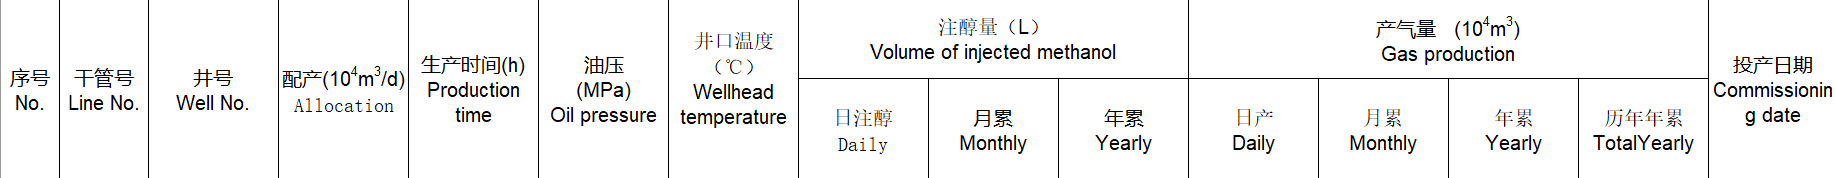
\includegraphics[scale=0.3,angle=0]{figure/表头1.png}
    \hfil
    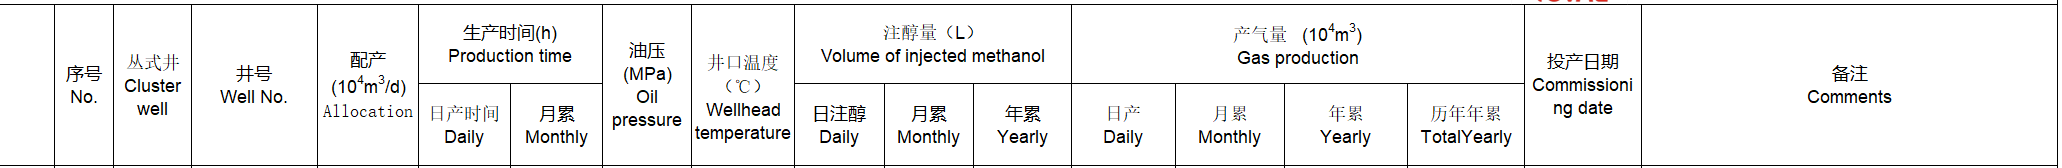
\includegraphics[scale=0.3,angle=0]{figure/表头2.png}
    \hfil
    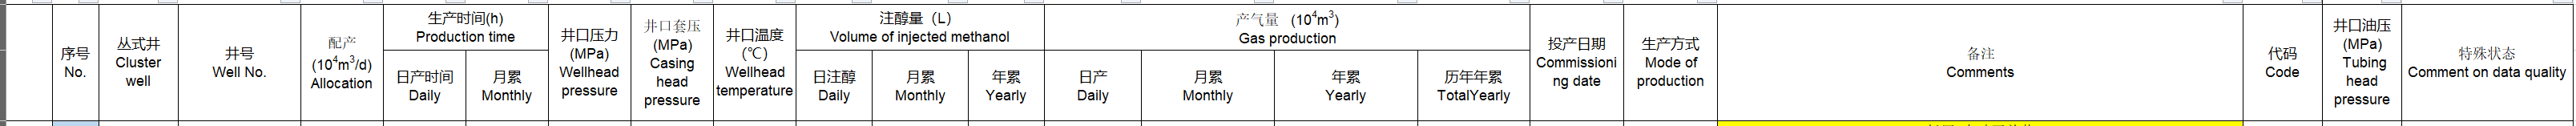
\includegraphics[scale=0.25,angle=0]{figure/表头3.png}
    \hfil
    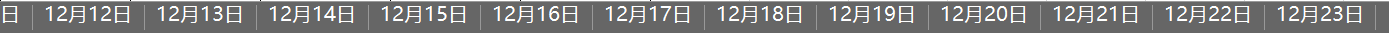
\includegraphics[scale=0.3,angle=0]{figure/日期格式1.png}
    \hfil
    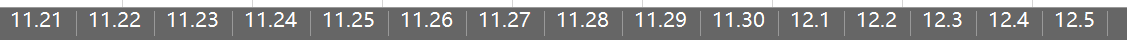
\includegraphics[scale=0.3,angle=0]{figure/日期格式2.png}
    \hfil
    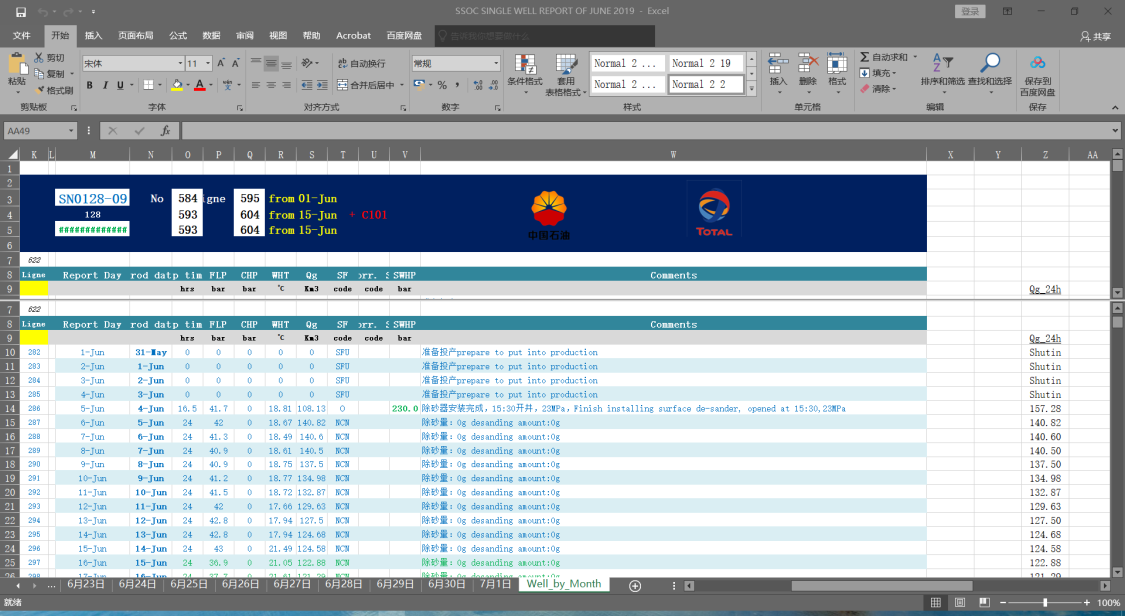
\includegraphics[scale=0.3,angle=0]{figure/总结性表.png}
    \caption{不同的表头、日期格式及总结性表}
    \label{fig:difTable}
\end{figure}

在进行原始数据的初步分析阶段,需要关注的数据列包括日期、集气站号、井序号、日产时间、井口压力(油压)、套压、井口温度、日产量和投产时间等关键指标。特别需要注意的是,套压数据的记录是从2016年9月开始的,这个时间点之前的数据中不包括套压信息。

在批量处理和读取原始数据的过程中,首先要去除每张Excel表中的冗余信息,这可能包括无关的汇总信息、非结构化的备注或者其他非目标数据列。随后,从每张表中提取出所需的关键列,这一步骤将会生成每个单井每日的数据记录,每天的记录将被整理并存储在一个单独的CSV格式文件中。预计在处理完整个时间范围后,将生成大约3664个此类文件,每个文件代表一个日报的数据集,覆盖从2012年8月3日至2022年8月15日的时间段。

合并多个日报数据集为一个单一数据集的过程包括一系列标准化和清洗步骤。首先,对于缺失的数据,例如某些日报可能缺少部分字段信息,需要进行合适的填充处理,比如使用前一天的数据或平均值等方法。接下来,对于数据格式的统一转换,所有的日期和时间字段应被转换成标准格式,比如ISO 8601标准的日期时间格式,而数值字段应确保为适当的数值类型,以便进行后续的分析和计算。

进一步,生成的所有单一日报数据集被合并成一个完整的数据集,以便进行全面的分析和模型训练。这个完整数据集,包含了所有气井在覆盖期内的所有记录,被存储在一个名为GasProductionOri.csv的文件中。但在这一大型数据集可以用于任何进一步分析之前,它需要经过详细的数据清洗过程。

数据清洗包括选择关键的数据子集、对列进行重命名以提高可读性和一致性、确保数据集按照时间顺序排列。此外,进行数据类型的统一化也是一个关键步骤,它包括将所有的日期和时间转换为统一的格式,确保所有的数值字段如日产量和井口压力都以一致的数据类型(如浮点数)来表示。

在实际数据中,可能会遇到一些特定的错误或异常值,如日产量异常低或异常高,或生产时间与日产量不匹配的情况。这些异常需要通过逻辑判断和上下文分析来纠正。例如,如果一个数据点显示日产量为0,但日开井时间为24小时,这显然是不合理的,应该根据实际情况调整。

最后,完成所有这些步骤后,还需进行一次最终的检查以确认数据集中没有重复的记录。通过识别和删除重复的条目,可以确保数据集的唯一性和准确性。完成所有这些数据处理步骤后,将得到一个干净、有序且格式统一的数据集,这个数据集可以被用于后续的数据分析、模型训练或其他数据驱动的任务中。
\begin{figure}[H]
    \centering
    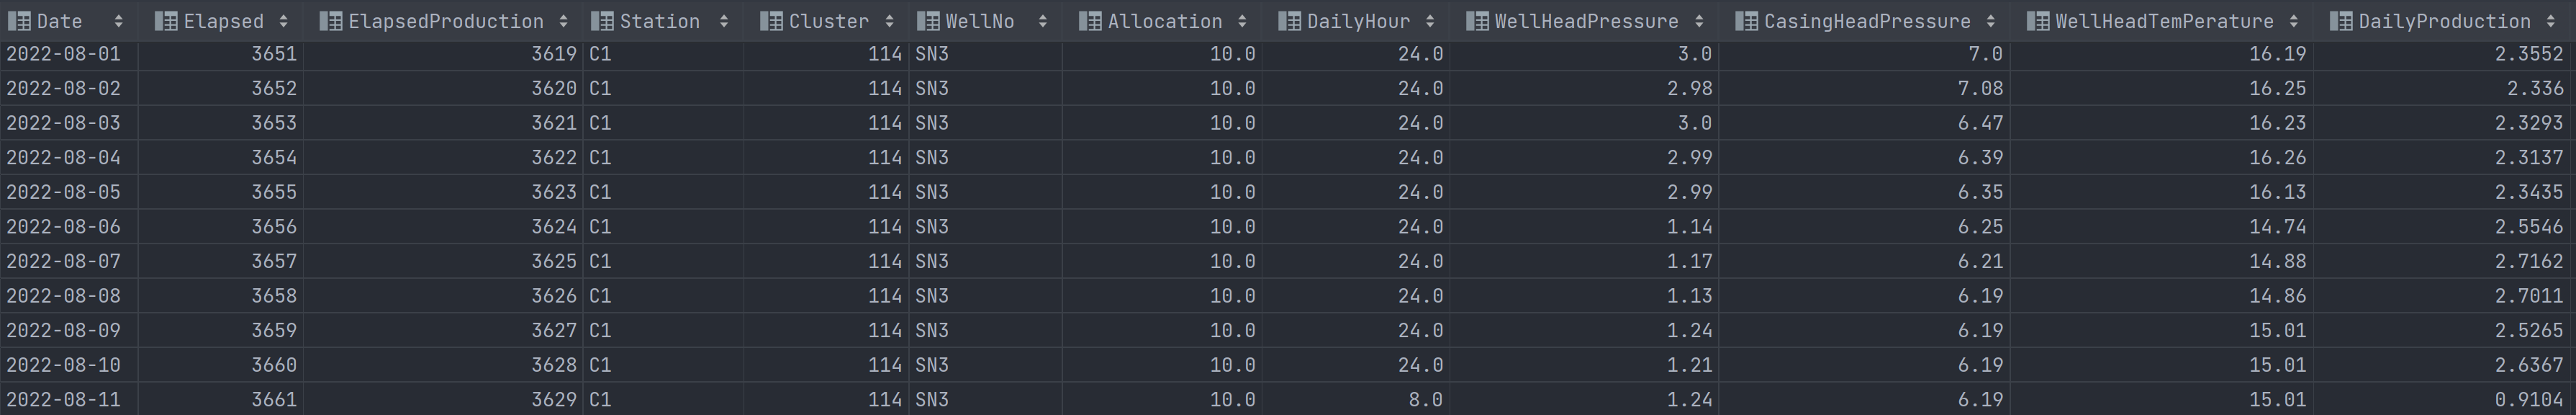
\includegraphics{figure/afterprocessdata.png}
    \caption{进行处理后的数据集示意图}
    \label{fig:afterprocess}
\end{figure}

剔除生产日期小于60天的井后,对其余井的历年累积产量,平均产量,峰值产量的进行统计分析,统计项包括计数,平均值,标准差,最小值,25\%分位数,中位数数,
75\%分位数,最大值,结果如下表所示,共910项数据。

\begin{figure}[H]
    \centering
    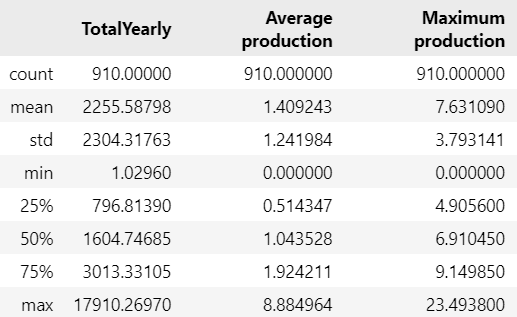
\includegraphics{figure/gasproduction.png}
    \caption{历年累积产量,平均产量,峰值产量的统计结果}
\end{figure}

为了便于分析和对比各气井的产量变化趋势及其随时间的动态变化,以及观察不同气井之间的时间序列曲线是否存在交叉点,本文计划制作一套交互式折线图。这些折线图将详细展示所有井的产气量随时间变化的趋势。

在这套交互式图表中,用户将有能力选择特定的井来查看其产量变化,这使得用户能够专注于分析特定井的性能,同时也可以轻松切换查看其他井的产量数据。此外,这种交互式设计还允许用户检查曲线上每个点的具体值,从而获得详细的日产量信息。

通过这种交互式的数据可视化方法,用户不仅可以直观地观察每口气井随时间的产量变化,还可以有效比较不同井之间的产量差异,以及识别任何可能的异常或显著的趋势变化。这种分析工具将大大增强数据的可访问性和可理解性,为气井的管理和优化提供有价值的洞察。
\begin{figure}[H]
    \centering
    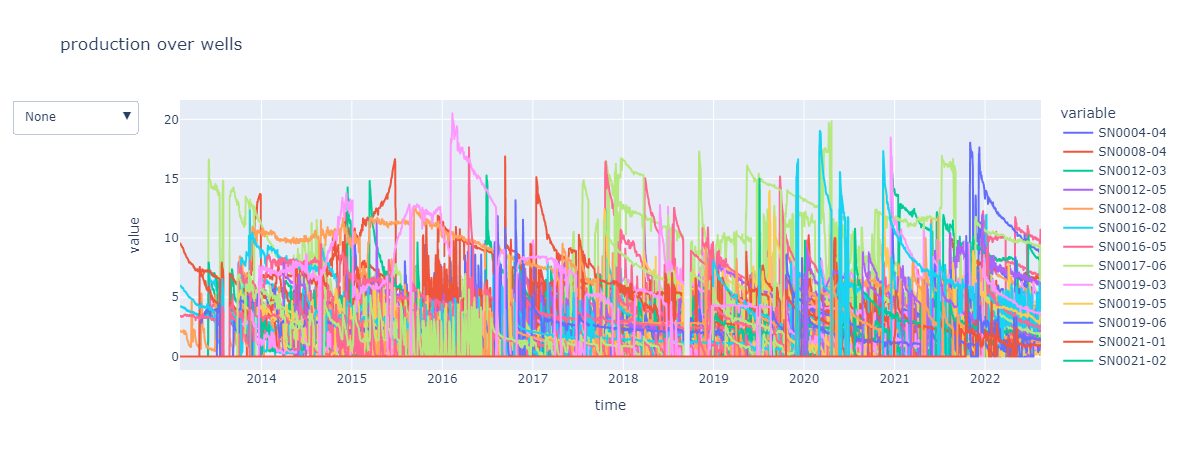
\includegraphics[scale=0.3,angle=0]{figure/productiongraph.png}
    \caption{在一张图上同时绘制多口井产量随时间的变化曲线}
    \label{fig:productionchange}
\end{figure}
\begin{figure}[H]
    \centering
    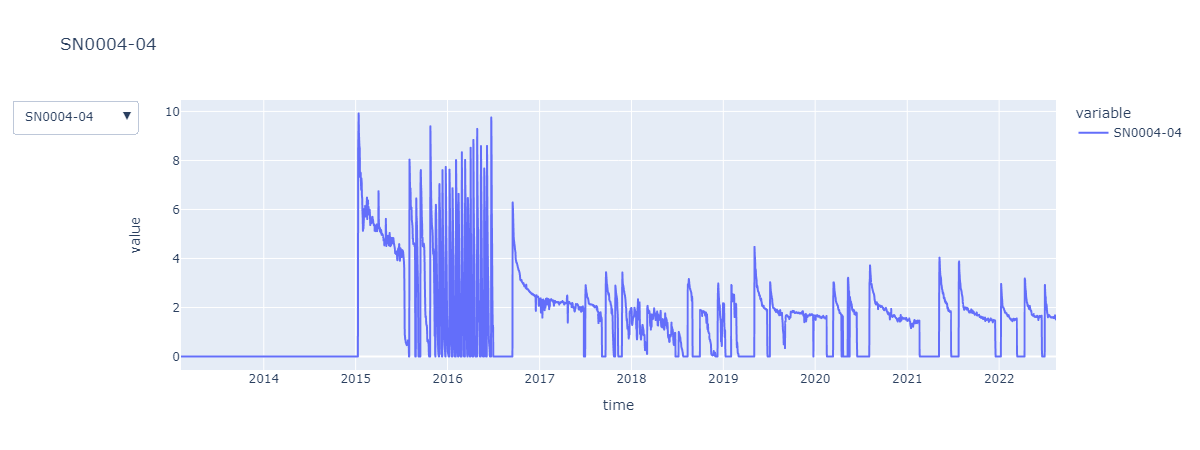
\includegraphics[scale=0.3,angle=0]{figure/awellgraph.png}
    \caption{井SN0004-04的产量随时间的变化曲线}
\end{figure}
\subsection{计算SBD距离}
由章节\ref{section2.1.1}可得,要计算SBD距离,需要先计算两条时间序列$x_t,y_t$之间的互相关$CC_w$,对互相关归一化得到$NCC_c$,根据最大的$NCC_c$计算两条序列
之间的SBD距离。再通过$NCC_c$取最大值(即$CC_w$值最大)时的w值减去$y_t$的长度来确定$y_t$与$x_t$最匹配时应该移动的步数。其算法如算法\ref{al:SBD}所示:
\begin{algorithm}[H]
    \caption{计算SBD距离以及与$y_t$对齐后的序列$y'_t$:$(\text{dist}, y'_t) = SBD(x_t, y_t)$}
    \begin{algorithmic}[1]
        \Require 两个归一化后的序列$x_t,y_t$
        \Ensure SBD距离dist,与$x_t$对齐后的序列$\hat{y}_t$
        \State 计算互相关值$CC_w(x_t, y_t) = F^{-1}(F(x_t) \times F(y_t))$\Comment{公式\eqref{eq:ccf}}%\eqref{eq:ccf}
        \State 对互相关值进行系数归一化$NCC_c = \frac{CC_w(x,y)}{\|x\|\|y\|}$
        \State $SBD(x_t, y_t) = 1 - \max_w \left( \frac{CC_w(x_t, y_t)}{\|x_t\| \cdot \|y_t\|} \right)$\Comment{公式\eqref{eq:SBD}}
        \State 计算$x_t,y_t$的长度$l_{y} = \text{length}(y_{t}),\text{length}(y_{t})$
        \State $y_t$的移动步数shift为$s = \text{which.max}(NCC) - l_y$
        \If{$s \geq 0$}:
            \State $\hat{y}_t = [\text{zeros}(0,s),y(1:l_x - s)]$\Comment{公式\eqref{eq:shift}}
        \Else:
            \State $\hat{y}_t = [y(1 - s:l_y),\text{zeros}(1,l_x - l_y - s)]$\Comment{公式\eqref{eq:shift}}
        \EndIf
    \end{algorithmic}
    \label{al:SBD}
\end{algorithm}  
\subsection{基于SBD距离的簇心提取}
根据章节\ref{section2.1.1}的介绍,求簇心需要得到$\mathbf{S} = \sum_{x_t \in P_k} x_t \cdot x_t^T$的最大特征值,此时$\mathbf{S}$最大特征值
对应的特征向量就是簇心对应的矩阵。其算法如算法\ref{al:center}所示:
\begin{algorithm}[H]
    \caption{根据当前聚类中心 $\mathbf{C}$ 和所有点 $\mathbf{X}$,计算更合理的聚类中心 $\mathbf{C'}$:$\mathbf{C'} = SE(\mathbf{C}, \mathbf{X})$}
    \begin{algorithmic}[1]
        \Require 簇内所有归一化之后的$n \times m$阶的时间序列矩阵$\mathbf{X}$;参考聚类中心$\mathbf{C}$
        \Ensure 新的聚类中心$\mathbf{C'}$
        \ForAll {$\mathbf{X}(i) \in \mathbf{X}$}
            \State 计算所有序列到中心的SBD距离以及与$x_t$对齐后的序列$x'_t$:$(\text{dist}, x'_t) = SBD(\mathbf{C}, x_t)$\Comment{算法\ref{al:SBD}}
            \State 由$x'_t$得到对齐后的序列矩阵$\mathbf{X'}$
        \EndFor
        \State 计算矩阵$\mathbf{S} = \mathbf{X}^T \cdot \mathbf{X}'$\Comment{公式\ref{eq:ckfin}中的$\mathbf{S}$}
        \State 对矩阵$\mathbf{S}$正则化后取其最大值对应的特征向量$\mathbf{C'}$
    \end{algorithmic}
    \label{al:center}
\end{algorithm}
\subsection{改进的k-Shape聚类}
与K-means相似,改进的K-Shape也通过迭代的方式不断更新聚类中心,并将对齐后的序列分配给各个簇心,直到迭代中心不再更新或者达到最大迭代次数为止。其过程
可以分为下面两步:

(1) 通过算法\ref{al:SBD}计算出的SBD距离,把数据分配给距离其最近的簇心;

(2) 根据(1)得到的聚类中心,通过算法\ref{al:center}计算新的聚类中心。

结合上文中的内容,最终改进的K-Shape算法如算法\ref{al:K-Shape}所示。
\begin{algorithm}[H]
    \caption{改进的K-Shape聚类}
    \begin{algorithmic}[1]
        \Require 归一化后样本集$\{x_1, x_2, \ldots, x_n\}$组成的$n \times m$阶时间序列矩阵$\mathbf{X}$,聚类簇数k
        \Ensure 各个样本所属的簇标记,$k \times m$阶簇心矩阵$\mathbf{C}$
        \State 根据章节\ref{sec:K-Shapeprocess}中的方法选取初始参考中心$c_j,j = 1, 2, \ldots, k$
        \While {聚类中心不再更新or迭代次数小于100:}
            \For {$i = 1, 2, \ldots, n$:} 
                \For {$j = 1, 2, \ldots, k$:}
                    \State 计算$SBD(c_j,x_i)$距离\Comment{算法\ref{al:SBD}}
                \EndFor
                \State 将$x_i$分配到距离其最近的中心所属的簇并将该簇所有序列记为矩阵$\mathbf{X_j}$
            \EndFor
            \For {$j = 1,2,\ldots,k$:}
                计算新聚类中心 $\mathbf{c_j}$:$\mathbf{c_j} = SE(\mathbf{c_j}, \mathbf{X_j})$\Comment{算法\ref{al:center}}
            \EndFor
        \EndWhile
    \end{algorithmic}
    \label{al:K-Shape}
\end{algorithm}
\section{实验对比分析}
\section{本章小结}